\section[Introducción]{Introducción}

\lipsum[1-3]
\lista{
    \item \lipsum[1]
    \item \lipsum[1]
}


\lipsum[1]

\subsection{Planteamiento del problema}

\lipsum[1-3]

\begin{table}[h!]
    \centering
    \begin{tabular}{rrr}
\toprule
 floor\_area &  year\_built &  nueva variable \\
\midrule
    61242.0 &      1942.0 &     118931964.0 \\
   274000.0 &      1955.0 &     535670000.0 \\
   280025.0 &      1951.0 &     546328775.0 \\
    55325.0 &      1980.0 &     109543500.0 \\
    66000.0 &      1985.0 &     131010000.0 \\
   119900.0 &      1956.0 &     234524400.0 \\
    91367.0 &      1982.0 &     181089394.0 \\
    50422.0 &      1947.0 &      98171634.0 \\
   122020.0 &      1929.0 &     235376580.0 \\
   102612.0 &      1979.0 &     203069148.0 \\
    65998.0 &      1979.0 &     130610042.0 \\
   100000.0 &      1927.0 &     192700000.0 \\
   128320.0 &      1960.0 &     251507200.0 \\
   616793.0 &      1955.0 &    1205830315.0 \\
    53000.0 &      1924.0 &     101972000.0 \\
    90045.0 &         NaN &             NaN \\
    74055.0 &      1949.0 &     144333195.0 \\
   128800.0 &      1926.0 &     248068800.0 \\
    91619.0 &      1914.0 &     175358766.0 \\
    53280.0 &      1973.0 &     105121440.0 \\
   217710.0 &      1900.0 &     413649000.0 \\
    68538.0 &      1913.0 &     131113194.0 \\
    90669.0 &      1962.0 &     177892578.0 \\
\bottomrule
\end{tabular}
    \caption{Consumo energético}
    \label{tab:my_label}
\end{table}

\begin{figure}[h!]
    \centering
    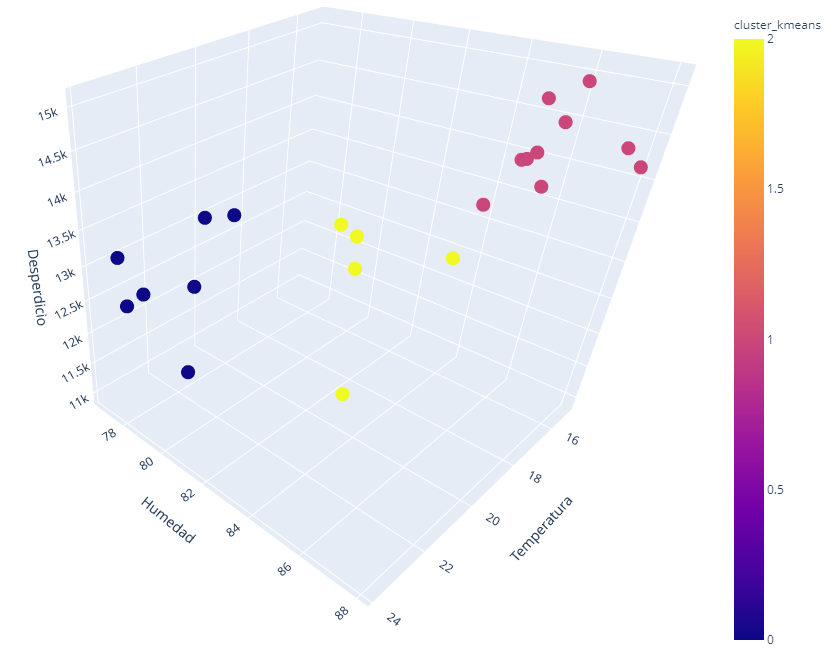
\includegraphics[width = 11cm]{figuras/cluster_3D.PNG}]
    \caption{Imagen de un cluster}
\end{figure}

\figura{5cm}{cluster_3D}{Ssoy una imagen de cluster\label{imagen_3D}}
\newpage
La imagen usando un algoritmo de machine learining del tipo K mean (ver figura \ref{imagen_3D})
